\chapter{Memory and Cache}
\label{c-cache}


\section{Memory}

2D

2.5D

A synchronous memory bus for a system with $2^k$ addresses of $n$ bit words would require at least:
\begin{itemize}
    \item k address lines
    \item n data lines
    \item 4+ control lines
\end{itemize}
or a total of $k+n+4$ parallel lines.  See Section~\ref{s-busses}

Memory is usually byte-addressable, but I don't just load it one byte at a time.  In a typical 2D or 2.5D RAM configuration though, if I had all of memory in one large module/array, I would only be able to access one byte at a time.  To allow access to more than one byte at a time, memory is interleaved: the first byte is stored in the first location of the first module/array, the second byte in the first location of the second module/array, and so on.  When all the module/arrays have their first location addressed, the second locations are specified, see Table~\ref{t-memadd}.

\begin{table}[h]
  \centering
  \begin{tabular}{|c|c|c|c|c|}
    \hline
    Module Address  & Module 1   & Module 2     & $\ldots$ & Module N \\ \hline
    $0$      & $0$        & $1$          & $\ldots$ & $N-1$    \\
    $1$      & $N$        & $N+1$        & $\ldots$ & $2N-1$   \\
    $\vdots$ & $\vdots$   & $\vdots$     & $\ddots$ & $\vdots$ \\
    $2^k-1$  & $(2^k-1)N$ & $(2^k-1)N+1$ & $\ldots$ & $2^kN-1$ \\ \hline
  \end{tabular}
  \caption{Mapping Memory Module's Addresses to the Computer's Memory Addresses}\label{t-memadd}
\end{table}

A number of potential problems can arise.  Consider the four byte integer, $0x12345678$, stored starting in address 2 on a machine with four modules.  In the easiest and fastest way to implement the hardware, the first byte of the returned number comes from the first module, the second byte from the second module and so on.  By examining Table~\ref{t-nonaligned} you will notice that this means the value sent back is $0x56781234$ or even $0xABCD1234$ depending on how the addresses are selected!

\begin{table}[h]
  \centering
  \begin{tabular}{|c|c|c|c|c|}
    \hline
    First Byte Address  & Module 1   & Module 2     & Module 3 & Module N \\ \hline
    $0$      & $0xAB$   & $0xCD$     & $0x12$   & $0x34$   \\
    $1$      & $0x56$   & $0x78$     & $0x00$   & $0x00$   \\ \hline
  \end{tabular}
  \caption{Memory Contents of Non-Aligned Integer}\label{t-nonaligned}
\end{table}

To prevent such problems, systems adopt standards of how memory must be stored.  The simplest method is justified, in which the first byte of any new memory item must start in the first module.  Justified can obviously lead to some inefficiencies in memory utilization.  A more sophisticated method is aligned, in which a new memory item must start at an address that is divisible by the number of bytes in the memory item (e.g.: a 4 byte integer can start at any address that can be expressed as $4i$ for $i$ a non-negative integer).

\subsection{Endian}

Big (LR) and little (RL) endian

Consistent (same for bits)

Sparc is inconsistent big-endian.

\begin{tabular}{ccc}
  % after \\: \hline or \cline{col1-col2} \cline{col3-col4} ...
  Endian & Consistent & Inconsistent \\
  \vspace{6pt}Big\vspace{6pt}    & \bigendianCon & \bigendianInc \\
  \vspace{6pt}Little\vspace{6pt} & \littleendianCon & \littleendianInc \\
\end{tabular}

\section{Cache Design}

In general DRAM has a cycle-time of about 50ns to 80ns, and SRAM has a cycle-time of 5ns to 20ns.  Main memory is almost exclusively DRAM due to size and cost, so access will be slow.  Strategies must be used to speed up access to main memory.  Several common techniques are:
\begin{description}
    \item[Wide Memory] memory that passes multiple words at a time.
    \item[Interleaving] memory that has successive addresses stored in different components that can be accessed simultaneously.
    \item[Prefetching] buffer that fetches most likely instructions (or sometimes data) when memory is idle.
    \item[Cache] data and instructions that have been accessed are stored in fast memory (SRAM) that is close to the CPU often as well as in main memory.
\end{description}
Usually, a variety of techniques are used, and often multiple levels of cache (l1, l2, and even l3).

Cache can be:
\begin{description}
    \item[fully associative] any main memory location can be stored in any cache location.
    \item[$2^k$-way set associative] each main memory location must be stored in one of n prescribed cache locations.  Usually, $16\geq k\geq 1$.
    \item[direct mapping] each main memory location must be stored in a particular cache location.  This is the same as 1-way set associative.
\end{description}

Let's introduce some formalisms.  Let $2^k$ be the associativity of the cache, $2^l$ be the size of a cache location (block size, usually less than 16 words), $2^m$ be the number of cache locations, and $2^n$ be the size of main memory.

Then
\beqn
\hbox{number of sets} &=& m-k \\
\hbox{size of the cache} &=& 2^{(l\times m)} \\
\hbox{\# address bits inferred by location} &=& m-k+l \\
\hbox{\# tag address bits} &=& n-(m-k+l)
\eeqn

\begin{tabular}{@{}clclclc@{}}
 & n-(m-k+l) && m-k && l & \\ \hline
\vline &  tag address bits & \vline & set address bits & \vline & offset in block & \vline \\ \hline
\end{tabular}

\vspace{.1in}
\Example{Cache for Toy Stack}

Design a 4 way associative, 8 byte cache for a 64 byte system (i.e.: the Toy Stack).  Show an example of how your system would do a cache lookup (ie: through all the steps for a lookup, you may pick memory and cache to have any values you want)

    {\color{ans}
    The numbers of our design are as follows.
    \begin{itemize}
        \item 64 bytes means 6 bit addresses
        \item 8 byte cache means 3 bit addresses
        \item 4 way associative means the high two bits of each cache address do not need to match the corresponding bits in main memory, but the least bit does.
        \item 5 bits of address from main memory need to be identified for each cache location, with the valid bit, this makes 6 tag bits for each cache location.
        \item the least significant bit of the main memory address to be checked for is used as a lookup on the cache to provided the 4 specific locations in cache that must be checked
        \item the 5 address tag bits of each of the 4 cache locations is compared with the high 5 bits of the main memory address.
        \item if any of them match and the corresponding valid bit is set then we have a cache hit and the data is sent
        \item if there is no match or the match is not valid main memory is accessed.
    \end{itemize}


    \textbf{lookup}

    Let the address to be checked for be $010111$, and let the cache be

    \begin{tabular}{|ccccc|c|ccc|c|}
      \hline
      \multicolumn{6}{|c|}{Tag Bits} & \multicolumn{3}{|c|}{Address} & Contents \\
      \multicolumn{5}{|c|}{High Address} & Valid Bit & \multicolumn{3}{|c|}{} &  \\
      \hline
      0 & 0 & 1 & 1 & 0 & 1 & 0 & 0 & 0 & 11011101 \\
      0 & 1 & 0 & 1 & 0 & 1 & 0 & 0 & 1 & 11010110 \\
      0 & 0 & 0 & 0 & 0 & 0 & 0 & 1 & 0 & 00011100 \\
      1 & 0 & 0 & 0 & 0 & 0 & 0 & 1 & 1 & 10010100 \\
      1 & 1 & 0 & 1 & 1 & 1 & 1 & 0 & 0 & 11101101 \\
      1 & 0 & 1 & 0 & 1 & 0 & 1 & 0 & 1 & 11011110 \\
      1 & 0 & 0 & 0 & 0 & 1 & 1 & 1 & 0 & 11111111 \\
      0 & 1 & 0 & 1 & 1 & 1 & 1 & 1 & 1 & 11010000 \\
      \hline
    \end{tabular}

    First, the low bit (a 1) of the address tells us to look at the 4 odd addresses in cache:

    \begin{tabular}{|ccccc|c|ccc|c|}
      \hline
      \multicolumn{6}{|c|}{Tag Bits} & \multicolumn{3}{|c|}{Address} & Contents \\
      \multicolumn{5}{|c|}{High Address} & Valid Bit & \multicolumn{3}{|c|}{} &  \\
      \hline
      0 & 1 & 0 & 1 & 0 & 1 & 0 & 0 & 1 & 11010110 \\
      1 & 0 & 0 & 0 & 0 & 0 & 0 & 1 & 1 & 10010100 \\
      1 & 0 & 1 & 0 & 1 & 0 & 1 & 0 & 1 & 11011110 \\
      0 & 1 & 0 & 1 & 1 & 1 & 1 & 1 & 1 & 11010000 \\
      \hline
    \end{tabular}

    The 5 address tag bits are checked against the high five bits of the address ($01011$):

    \begin{tabular}{|ccccc|c|ccc|c|}
      \hline
      \multicolumn{6}{|c|}{Tag Bits} & \multicolumn{3}{|c|}{Address} & Contents \\
      \multicolumn{5}{|c|}{High Address} & Valid Bit & \multicolumn{3}{|c|}{} &  \\
      \hline
      0 & 1 & 0 & 1 & 1 & 1 & 1 & 1 & 1 & 11010000 \\
      \hline
    \end{tabular}

    The address matches and the valid bit is set so $11010000$ is sent as the contents.

    }


\vspace{.1in}
\Example{8-way set associative}

Consider a machine with 32 bit addressing (up to 4GB of RAM) and 512k ($2^{19}$) of data cache with 1 byte blocks.  To define the 8-way set association, it will be required that main memory addresses must have the same last 16 bits (19-3=16) as a cache location to be stored in that cache location.  Every cache location has 17 extra bits, 16 for addressing, and one for validity.  Eight location in cache must be checked for each main memory access (it is 8-way for a reason).  The main memory address to be checked is split into the upper and lower 16 bits.  The lower 16 bits are used to identify the eight cache locations, whose 16 address tag bits are then compared to the 16 high bits of the main memory address, see Figure~\ref{f-8wsac}.  This generates eight signals (true if match was found) that are then logically and'ed together with the corresponding 8 validity bits (might have the same address but might not be current).  If any generates a hit (is true) then its contents are sent as the data.

\begin{figure}
  % Requires \usepackage{graphicx}
  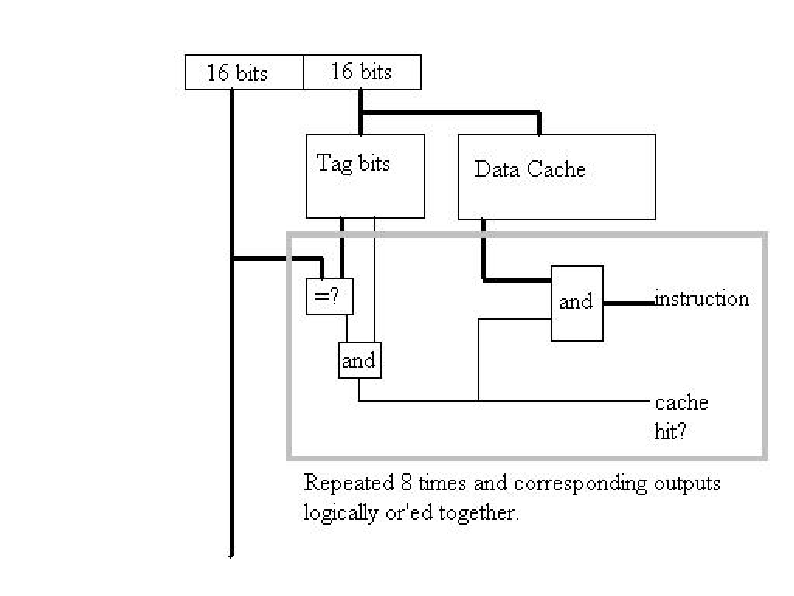
\includegraphics[width=4in]{cache.png}\\
  \caption{8-Way Set Associative Cache}\label{f-8wsac}
\end{figure}

Replacement policies
\begin{description}
    \item[LRU] Least Recently Used
    \item[FIFO] First-in First-out
    \item[LFU] Least Frequently Used
    \item[Random] Random
\end{description}

\subsection{Neat Little LRU Algorithm}

Let the number of cache slots (locations) be $2^k$, then we create a matrix of bits that is $2^k\times 2^k$ (so we can associate the cache address with both a row and column).  Initially they are all cleared.  When a cache slot, say address $p$, is accessed:
\begin{enumerate}
    \item $1$'s are placed in every bit of the matrix row $p$,
    \item $0$'s are placed in every bit of the matrix column $p$.
\end{enumerate}
Note that the second step will delete one of the $1$'s you placed in the first step.

The the address that was least recently used corresponds to the number of the row that has a sum of zero.  Equivalently, the address that was least recently used corresponds to the number of the column with the largest sum.

\Example{Fully Associative Cache With 4 Slots}

For simplicity we will assume main memory has 256 ($2^8$) bytes, and the data length is 1 byte.  The cache starts empty.

\vspace{6pt}\noindent
\begin{tabular}{|c|c|c|c|c|c|c|c|}
  \hline
  \multicolumn{4}{|c|}{NLLRU} & \multicolumn{3}{|c|}{Tag Bits} & Data \\
  0 & 1 & 2 & 3 & V & D & Address & \\ \hline
  0 & 0 & 0 & 0 & 0 & 0 & 0x00 & 0x00 \\
  0 & 0 & 0 & 0 & 0 & 0 & 0x00 & 0x00 \\
  0 & 0 & 0 & 0 & 0 & 0 & 0x00 & 0x00 \\
  0 & 0 & 0 & 0 & 0 & 0 & 0x00 & 0x00 \\
  \hline
\end{tabular}
\vspace{6pt}

Address 0x1A, which contains 0x49, is accessed.

\vspace{6pt}\noindent
\begin{tabular}{|c|c|c|c|c|c|c|c|}
  \hline
  \multicolumn{4}{|c|}{NLLRU} & \multicolumn{3}{|c|}{Tag Bits} & Data \\
  0 & 1 & 2 & 3 & V & D & Address & \\ \hline
  0 & 1 & 1 & 1 & 1 & 0 & 0x1A & 0x49 \\
  0 & 0 & 0 & 0 & 0 & 0 & 0x00 & 0x00 \\
  0 & 0 & 0 & 0 & 0 & 0 & 0x00 & 0x00 \\
  0 & 0 & 0 & 0 & 0 & 0 & 0x00 & 0x00 \\
  \hline
\end{tabular}
\vspace{6pt}

Address 0x05, which contains 0x11, is accessed.

\vspace{6pt}\noindent
\begin{tabular}{|c|c|c|c|c|c|c|c|}
  \hline
  \multicolumn{4}{|c|}{NLLRU} & \multicolumn{3}{|c|}{Tag Bits} & Data \\
  0 & 1 & 2 & 3 & V & D & Address & \\ \hline
  0 & 0 & 1 & 1 & 1 & 0 & 0x1A & 0x49 \\
  1 & 0 & 1 & 1 & 1 & 0 & 0x05 & 0x11 \\
  0 & 0 & 0 & 0 & 0 & 0 & 0x00 & 0x00 \\
  0 & 0 & 0 & 0 & 0 & 0 & 0x00 & 0x00 \\
  \hline
\end{tabular}
\vspace{6pt}

Address 0x25, which contains 0xFF, is accessed.

\vspace{6pt}\noindent
\begin{tabular}{|c|c|c|c|c|c|c|c|}
  \hline
  \multicolumn{4}{|c|}{NLLRU} & \multicolumn{3}{|c|}{Tag Bits} & Data \\
  0 & 1 & 2 & 3 & V & D & Address & \\ \hline
  0 & 0 & 0 & 1 & 1 & 0 & 0x1A & 0x49 \\
  1 & 0 & 0 & 1 & 1 & 0 & 0x05 & 0x11 \\
  1 & 1 & 0 & 1 & 0 & 0 & 0x25 & 0xFF \\
  0 & 0 & 0 & 0 & 0 & 0 & 0x00 & 0x00 \\
  \hline
\end{tabular}
\vspace{6pt}

The value 0x33 is stored to address 0x05.

\vspace{6pt}\noindent
\begin{tabular}{|c|c|c|c|c|c|c|c|}
  \hline
  \multicolumn{4}{|c|}{NLLRU} & \multicolumn{3}{|c|}{Tag Bits} & Data \\
  0 & 1 & 2 & 3 & V & D & Address & \\ \hline
  0 & 0 & 0 & 1 & 1 & 0 & 0x1A & 0x49 \\
  1 & 0 & 1 & 1 & 1 & 1 & 0x05 & 0x33 \\
  1 & 0 & 0 & 1 & 0 & 0 & 0x25 & 0xFF \\
  0 & 0 & 0 & 0 & 0 & 0 & 0x00 & 0x00 \\
  \hline
\end{tabular}
\vspace{6pt}

The value 0xF5 is stored to address 0x06.

\vspace{6pt}\noindent
\begin{tabular}{|c|c|c|c|c|c|c|c|}
  \hline
  \multicolumn{4}{|c|}{NLLRU} & \multicolumn{3}{|c|}{Tag Bits} & Data \\
  0 & 1 & 2 & 3 & V & D & Address & \\ \hline
  0 & 0 & 0 & 0 & 1 & 0 & 0x1A & 0x49 \\
  1 & 0 & 1 & 0 & 1 & 1 & 0x05 & 0x33 \\
  1 & 0 & 0 & 0 & 0 & 0 & 0x25 & 0xFF \\
  1 & 1 & 1 & 0 & 1 & 1 & 0x06 & 0xF5 \\
  \hline
\end{tabular}
\vspace{6pt}

The value 0x07 is stored to address 0x07.

\vspace{6pt}\noindent
\begin{tabular}{|c|c|c|c|c|c|c|c|}
  \hline
  \multicolumn{4}{|c|}{NLLRU} & \multicolumn{3}{|c|}{Tag Bits} & Data \\
  0 & 1 & 2 & 3 & V & D & Address & \\ \hline
  0 & 1 & 1 & 1 & 1 & 1 & 0x07 & 0x07 \\
  0 & 0 & 1 & 0 & 1 & 1 & 0x05 & 0x33 \\
  0 & 0 & 0 & 0 & 0 & 0 & 0x25 & 0xFF \\
  0 & 1 & 1 & 0 & 1 & 1 & 0x06 & 0xF5 \\
  \hline
\end{tabular}
\vspace{6pt}

\subsection{Implementing LRU Algorithm}

NLLRU is a nice algorithm to learn off, but it is not a good one to build.  First off it requires over twice as many bits as is needed.  Second, it can become inconsistent if a bit flip occurs.  To understand these problems notice the LRU square is skew symmetric:
\begin{enumerate}
\item The main diagonal is always zero.
\item The lower triangular elements (lower left triangle of the LRU square) are the negated transpose (each bit is the logical not of the bit on the opposite side of the main diagonal) of the upper triangular elements (upper right triangle of the LRU square.
\end{enumerate}

\subsection{Cache Performance}

We will be concerned with some basic numbers
\begin{description}
    \item[Hit Ratio (HR)] The number of cache hits over the number of lookups.
    \item[Miss Ratio (MR)] The number of cache misses over the number of lookups.
    \item[Effective Access Time (EAT or $T_{eff}$)] The average time spent in a memory access.
\end{description}

First let us consider the hit and miss ratios.  For a series of lookups, the number of hits was ``$Hit$" and the number of misses was ``$Miss$", thus $Hit+Miss=lookups$.  Given this,
\begin{eqnarray*}
  HR &=& \frac{Hit}{Hit+Miss} \\
  MR &=& \frac{Miss}{Hit+Miss} \\
  1 &=& HR+MR
\end{eqnarray*}

thus,

\begin{eqnarray*}
  T_{eff} &=& \frac{Hit\times T_{Hit}+Miss\times T_{Miss}}{Hit+Miss} \\
          &=& HR\times T_{Hit}+MR\times T_{Miss}.
\end{eqnarray*}

Usually, the miss time is the access time ($T_{Hit}$), plus a miss penalty (say $T_{Penalty}$).

\begin{eqnarray*}
  T_{Miss}&=& T_{Hit}+T_{Penalty} \\
  T_{eff} &=& HR\times T_{Hit}+MR\times T_{Miss} \\
          &=& HR\times T_{Hit}+MR\times (T_{Hit}+T_{Penalty}) \\
          &=& (HR+MR)\times T_{Hit}+MR\times T_{Penalty} \\
          &=& T_{Hit}+MR\times T_{Penalty}
\end{eqnarray*}





\vspace{.1in}\noindent
\textbf{Example}


Use the following chart to show the state of a 4 location, 2-Way associative cache, that uses LRU.  If a location has a number printed in it, the address is valid, if no number appears the contents are invalid.  For simplicity the computer only has 16 locations in memory.  If the cache takes 5ns to access and RAM takes 60ns, what is the effective access time given the sequence?

\begin{tabular}{|l|c|c|c|c|c|c|c|c|c|c|c|} \hline
Time              & 0 & 1 & 2 & 3 & 4 & 5 & 6 & 7 & 8 & 9 & 10 \\ \hline
Lookup Address    & - & 2 & 5 & 6 & B & 5 & 2 & 2 & B & C & 5  \\ \hline
Cache location 00 & A &   &   &   &   &   &   &   &   &   &    \\ \hline
Cache location 01 & B &   &   &   &   &   &   &   &   &   &    \\ \hline
Cache location 10 &   &   &   &   &   &   &   &   &   &   &    \\ \hline
Cache location 11 &   &   &   &   &   &   &   &   &   &   &    \\ \hline
\end{tabular}

{\color{ans}
\begin{tabular}{|l|c|c|c|c|c|c|c|c|c|c|c|} \hline
Time              & 0 & 1 & 2 & 3 & 4 & 5 & 6 & 7 & 8 & 9 & 10 \\ \hline
Lookup Address    & - & 2 & 5 & 6 & B & 5 & 2 & 2 & B & C & 5  \\ \hline
Cache location 00 & A & A & A & 6 & 6 & 6 & 6 & 6 & 6 & C & C  \\ \hline
Cache location 01 & B & B & B & B & B & B & B & B & B & B & B  \\ \hline
Cache location 10 &   & 2 & 2 & 2 & 2 & 2 & 2 & 2 & 2 & 2 & 2  \\ \hline
Cache location 11 &   &   & 5 & 5 & 5 & 5 & 5 & 5 & 5 & 5 & 5  \\ \hline
\end{tabular}

MR=.4

\beqn
T_{eff}
 &=& T_{cache}+MR(T_{RAM}) \\
 &=& 5 ns+.4(60 ns) \\
 &=& 29 ns
\eeqn
}



\section{Virtual Memory}

A 32-bit virtual memory system has a 64KB page size, and 1 GB of RAM.  How large is the physical page number in bits? Assuming that the each entry in the table is word aligned, how large is the lookup table in bytes?

{\color{ans}
64KB = $2^{16}$

1GB = $2^{30}$

So the physical page number takes 30-16=14 bits or almost 2B to store in the table.  We also need to add memory protection, ownership, validity, location, etc.  I will assume that I can fit all this in 4B.

The table size is $2^{(32-16)}\times 4 B = 2^{18} B = 256 KB$
} 